%\part{Metodologia}

\chapter[Metodologia]{Metodologia}

Na aplicação do método científico deve-se explicitar por quais meios, métodos e ferramentas foram usadas para os testes e provas da pesquisa que o projeto está direcionado. Com isso o pesquisador reune informações que podem ou não corroborar com a sua tese inicial. O principal método do projeto foi o \textit{Top Down}, onde os subsistemas que formam o projeto foram divididos entre os integrantes da equipe.

\section{Metodologia Top Down}

\textit{Top Down} significa "de cima para baixo" e é uma maneira de organizar um projeto dividindo a lógica ou blocos funcionais dele em partes menores e com funções mais específicas que, quando unidos, formam o projeto completo. Resumindo é um método que visa a arquitetura da gestão que começa por uma abordagem geral e desce até níveis específicos.\cite{site_top_down}

Na equipe, os blocos foram divididos entre os membros para o  desenvolvimento como exibido na Fig. \ref{fig03}. Na Fig. \ref{fig02} observa-se o topo da montagem com a relação entre os blocos, que serão 5: o retificador, o tensão de referência, o LDO, o conversor tensão frequência e o transmissor UWB.

\begin{figure}[htb]
	\centering
	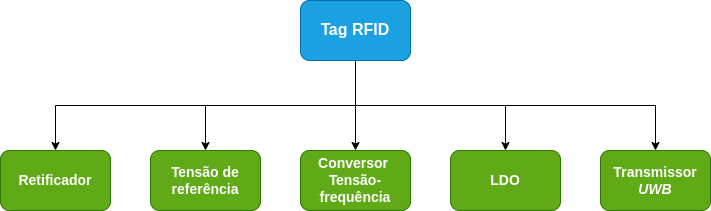
\includegraphics[width=0.6\textwidth]{figuras/diagrama.png}
	\caption{Diagrama de blocos dos módulos Top-Down em desenvolvimento}
	\label{fig03}
\end{figure}


\begin{figure}[htb]
	\centering
	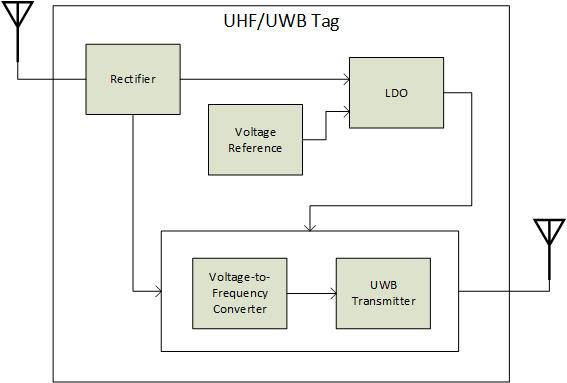
\includegraphics[width=0.6\textwidth]{figuras/Top.jpg}
	\caption{Visão do \textit{Top Module} da \textit{Tag RFID} desenvolvida no projeto. Fonte:\cite{artigo_tag_unb} }
	\label{fig02}
\end{figure}



\section{Simulações Cadence Virtuoso }

A ferramenta usada na confecção e simulação dos circuitos foi o Cadence Virtuoso com a licença disponibilizada à UnB para uso dos alunos e professores para projetos de CIs. Ela foi usada desde o início das simulações não tendo outra IDE ou programa alternativo para simulação de circuitos anterior ou posterior à escolha dela.

Sua escolha tem como principal razão o uso da tecnologia \textit{UMC 018$\mu$} para a fabricação de CIs, que foi a base para o projeto e criação da \textit{TAG}. 




